\part{Foundations}

\section{Neural networks in five minutes}
\markboth{Neural networks}{Neural networks}

\subsection{What a network is, for this project}
An image classifier such as ResNet8 takes a picture and outputs a list of scores, one per class
(``airplane'', ``cat'', and so on). The class with the highest score is the prediction. Everything the
network knows is stored in numbers:
\begin{itemize}
\item \term{Weights} are fixed numbers learned during training. A small ResNet8 has about 78{,}000 of them,
 RepVGG-A0 about 7 million, your vision transformer about 2.7 million. They sit in memory the whole time
 the network is deployed.
\item \term{Activations} are temporary numbers. When one picture goes through the network, every layer
 computes new values from the previous layer's values. These are held in buffers just for that one picture.
\end{itemize}
A \term{layer} (a convolution or a fully connected layer) multiplies its input activations by its weights
and adds the results. Many layers stacked make the network.

\subsection{Training versus inference}
\term{Training} adjusts the weights so predictions become correct. \term{Inference} means using the finished
network to classify new pictures. Your whole project is about inference: you train a network once, then
study what happens when stored values are corrupted while it is being used.

\subsection{Words you will see all the time}
\begin{description}[leftmargin=2.2cm,style=nextline]
\item[Top-1 accuracy] The fraction of test pictures where the highest-scoring class is the correct one.
\item[Logits] The raw output scores, one per class, before any normalisation.
\item[Margin] The gap between the highest and the second-highest logit for one picture,
 $m = z_{(1)} - z_{(2)}$. A small margin means the network is nearly undecided between two classes.
 This quantity turns out to matter a great deal in your results.
\item[Prediction changed] A picture whose predicted class differs from what the fault-free network predicted
 (not from the true label). Your project measures how often a fault changes predictions.
\item[Seed] A number that fixes the random choices made during training (starting weights, order of
 pictures). Two networks with the same design and different seeds are two different trained networks that
 reach nearly the same accuracy but differ in many details. Seeds matter a lot later.
\item[CIFAR-10 / CIFAR-100] Small image datasets: $32\times32$ colour pictures. CIFAR-10 has 10 classes
 (60{,}000 images), CIFAR-100 has 100 classes with ten times fewer images per class, so it is a harder task.
\end{description}

\subsection{The three networks you used}
\begin{itemize}
\item \textbf{ResNet8}: the MLPerf Tiny image-classification network. A $3\times3$ convolution at the start
 (the ``stem''), three residual blocks, and a linear layer at the end: eight weight layers on the main path
 plus two $1\times1$ shortcut convolutions, ten quantised layers in all. At width 16 it has 78{,}042
 parameters. ``Width'' is the number of channels in the first layer; you trained widths 8, 16, 24, 32, 48
 (20 thousand to 692 thousand parameters).
\item \textbf{RepVGG-A0}: a plain stack of $3\times3$ convolutions. During training each block has three
 parallel branches ($3\times3$, $1\times1$, identity); for deployment the branches are fused into one
 $3\times3$ convolution. About 7.0 million parameters after fusion.
\item \textbf{A small Vision Transformer (ViT)}: the width and head count of DeiT-Tiny (192 dimensions,
 3 heads), depth 6, $4\times4$ patches, 2.7 million parameters. DeiT is the transformer family used in
 the TreeFI paper and named in your proposal; yours is a smaller version trained from scratch on CIFAR.
\end{itemize}

\section{Numbers inside a computer}
\markboth{Numbers in a computer}{Numbers in a computer}

\subsection{Bits}
A \term{bit} is a 0 or a 1. A number is stored as a row of bits. $n$ bits can name $2^n$ different things:
8 bits give 256 codes, 6 bits give 64, 4 bits give 16.

\subsection{FP32, the normal format}
Ordinary computation uses \term{FP32} (32-bit floating point), laid out as
\[
\underbrace{1}_{\text{sign}}\;|\;\underbrace{8}_{\text{exponent}}\;|\;\underbrace{23}_{\text{mantissa}}.
\]
The value is $(-1)^{\text{sign}}\times(1+\text{mantissa}/2^{23})\times2^{\text{exponent}-127}$. It is scientific
notation in base 2: the exponent says how big the number is, the mantissa says exactly where inside that size.
Every FP32 number is \emph{self-contained}: all its information lives in its own 32 bits. So if one bit of a
FP32 weight flips, exactly that one weight changes.

\subsection{Why shrink the numbers: quantisation}
32 bits per weight is a lot of memory, and moving memory costs energy and time. \term{Quantisation} stores
each number in fewer bits (8, 6 or 4) at the price of rounding error. A quantised network is slightly
different from the original, but if it is done well, accuracy barely changes.

\subsection{Fake quantisation, which is what your tool does}
Your tool runs everything in FP32 on a normal PC, but \emph{before} using a weight it rounds it to the value
the MX format could actually store. This is called \term{fake quantisation}: the network computes with exactly
the numbers an MX accelerator would use, though the arithmetic is done in FP32. Faults are injected in the
stored bit pattern, then decoded to FP32 and used.

\section{Microscaling (MX) formats}
\markboth{Microscaling}{Microscaling}

\subsection{The idea}
MX is defined by the OCP Microscaling Formats specification (and the paper by Rouhani et al., 2023). Group the
numbers of a tensor into \term{blocks} of $K$ consecutive numbers (usually $K=32$). For each block store
\begin{itemize}
\item one \term{shared scale} $X$: 8 bits, shared by all $K$ numbers; and
\item one small \term{element code} per number: 4, 6 or 8 bits.
\end{itemize}
The real value of element $i$ is
\begin{equation}\label{eq:mx}
v_i \;=\; \operatorname{decode}(\text{code}_i)\;\times\;2^{\,X-127}.
\end{equation}

\begin{plain}
Think of a price list of 32 items with one note at the top: ``all prices in thousands''. Each row only
stores a short number, and the single note says how to read all of them. That saves a lot of memory. The
danger is obvious: if the note gets corrupted, \emph{all 32 prices} become wrong at once.
\end{plain}

\subsection{The scale is E8M0}
The scale byte is in a format called \term{E8M0}: 8 exponent bits and no mantissa bits. So the scale is always
an exact power of two: byte $X$ means $2^{X-127}$. Byte 127 means $\times1$, byte 128 means $\times2$, byte 118
means $2^{-9}$. Bytes 0 to 254 are normal scales (so the range is $2^{-127}$ to $2^{127}$). \textbf{Byte 255 is
reserved to mean NaN} (not a number, an error value).

\subsection{Memory saved}
A block of 32 numbers with 8-bit codes needs $8+32\times8=264$ bits, which is $8.25$ bits per number instead
of 32. That is the benefit.

\subsection{Two fault sites and the blast radius}
This is the central structural fact of your project (it comes straight from your proposal).
\begin{center}
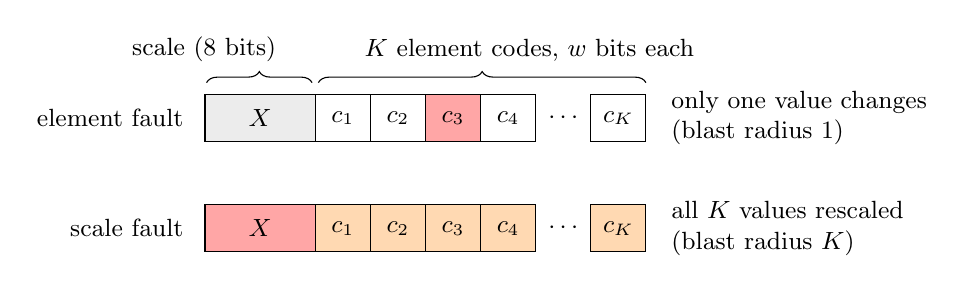
\begin{tikzpicture}[font=\small,
  cell/.style={draw, minimum width=7mm, minimum height=6mm, inner sep=0pt},
  scl/.style={draw, minimum width=14mm, minimum height=6mm, inner sep=0pt}]
  \node[anchor=east] at (-0.15,0) {element fault};
  \node[scl, fill=gray!15] at (0.7,0) {$X$};
  \node[cell] at (1.75,0) {$c_1$};
  \node[cell] at (2.45,0) {$c_2$};
  \node[cell, fill=red!35] at (3.15,0) {$c_3$};
  \node[cell] at (3.85,0) {$c_4$};
  \node at (4.55,0) {$\cdots$};
  \node[cell] at (5.25,0) {$c_K$};
  \node[anchor=west, align=left] at (5.8,0) {only one value changes\\(blast radius 1)};
  \node[anchor=east] at (-0.15,-1.4) {scale fault};
  \node[scl, fill=red!35] at (0.7,-1.4) {$X$};
  \foreach \x/\l in {1.75/c_1,2.45/c_2,3.15/c_3,3.85/c_4,5.25/c_K}
     \node[cell, fill=orange!30] at (\x,-1.4) {$\l$};
  \node at (4.55,-1.4) {$\cdots$};
  \node[anchor=west, align=left] at (5.8,-1.4) {all $K$ values rescaled\\(blast radius $K$)};
  \draw[decorate, decoration={brace, amplitude=4pt}] (0.02,0.45) -- (1.36,0.45)
    node[midway, above=4pt, xshift=-7mm] {scale (8 bits)};
  \draw[decorate, decoration={brace, amplitude=4pt}] (1.44,0.45) -- (5.6,0.45)
    node[midway, above=4pt, xshift=6mm] {$K$ element codes, $w$ bits each};
\end{tikzpicture}
\captionof{figure}{One MX block and its two fault sites. Red is the flipped word; orange are the values it changes.}
\end{center}

A flip of bit $j$ of the scale multiplies every value in the block by $2^{\pm2^{j}}$: bit 0 means $\times2$ or
$\div2$, bit 1 means $\times4$, bit 2 means $\times16$, bit 3 means $\times256$, \ldots, bit 7 means $\times2^{128}$.
That is why the scale is so dangerous.

\src{proposal PDF Sec.~1 and 3; mxfi/formats.py (E8M0 definition); report Sec.~2.}

\section{The five element formats}
\markboth{Element formats}{Element formats}

\subsection{Anatomy of an element code}
An element code has three groups of bits. Names such as \ee{e4m3} mean: \textbf{e}xponent \textbf{4} bits,
\textbf{m}antissa \textbf{3} bits, plus one sign bit, 8 bits in all. The names MXFP8, MXFP6 and MXFP4
count the total bits per element.

\begin{center}
\begin{tikzpicture}[font=\small, bit/.style={draw, minimum width=8mm, minimum height=7mm, inner sep=0pt}]
  \foreach \i/\v in {0/0,1/1,2/1,3/1,4/0,5/0,6/1,7/0}{
    \node[bit] at (\i*0.85,0) {\v};
  }
  \foreach \i/\b in {0/7,1/6,2/5,3/4,4/3,5/2,6/1,7/0}{
    \node[font=\scriptsize, text=srcc] at (\i*0.85,0.65) {bit \b};
  }
  \draw[decorate,decoration={brace,mirror,amplitude=3pt}] (-0.4,-0.5) -- (0.4,-0.5) node[midway,below=3pt] {sign};
  \draw[decorate,decoration={brace,mirror,amplitude=3pt}] (0.45,-0.5) -- (3.8,-0.5) node[midway,below=3pt] {exponent (4 bits)};
  \draw[decorate,decoration={brace,mirror,amplitude=3pt}] (3.85,-0.5) -- (6.35,-0.5) node[midway,below=3pt] {mantissa (3 bits)};
\end{tikzpicture}
\captionof{figure}{The bits of an \ee{e4m3} code; the example shown is \ee{01110010}.}
\end{center}

\subsection{Decoding a code by hand}
For a code with exponent field $e$ and mantissa field $f$ (an $M$-bit number), when $e\neq0$:
\begin{equation}\label{eq:decode}
\operatorname{decode}=(-1)^{s}\,\Bigl(1+\frac{f}{2^{M}}\Bigr)\,2^{\,e-\mathrm{bias}},\qquad
\mathrm{bias}=2^{\text{exp\_bits}-1}-1 .
\end{equation}
When $e=0$ the number is \term{subnormal}: there is no leading ``1+'', which is how the format gets zero and very
tiny numbers.

\begin{worked}[Worked example: decode the e4m3 code 01110010]
Sign bit $=0$ (positive). Exponent bits \ee{1110} $=14$. Mantissa bits \ee{010} $=2$, with $M=3$. The bias of
e4m3 is $2^{3}-1=7$. So
\[
\Bigl(1+\tfrac{2}{8}\Bigr)\times2^{14-7}=1.25\times128=\mathbf{160}.
\]
The table inside \code{mxfi/formats.py} also gives 160.0 (checked by running it).
\end{worked}

\subsection{What bias is}
The exponent field only stores $0,1,2,\dots$, but we need small numbers like $2^{-3}$ too. So the stored value means
``exponent plus bias'', and the bias (7 for e4m3, 15 for e5m2, 3 for e3m2, 1 for e2m3 and e2m1) is subtracted
back out.

\subsection{The smallest format on one card: e2m1}
The 4-bit format has only 16 codes. All of them (computed from your \code{formats.py}):
\begin{center}
\small
\begin{tabular}{cc@{\hspace{2cm}}cc}
\toprule
code & value & code & value \\
\midrule
0000 & 0 & 1000 & $-0$ \\
0001 & 0.5 & 1001 & $-0.5$ \\
0010 & 1 & 1010 & $-1$ \\
0011 & 1.5 & 1011 & $-1.5$ \\
0100 & 2 & 1100 & $-2$ \\
0101 & 3 & 1101 & $-3$ \\
0110 & 4 & 1110 & $-4$ \\
0111 & \textbf{6} & 1111 & $-6$ \\
\bottomrule
\end{tabular}
\end{center}
With 4 bits you can only say $0, 0.5, 1, 1.5, 2, 3, 4, 6$ and their negatives. That is why the largest value is 6.
The shared scale then slides this tiny menu up or down to wherever the real weights are.

\subsection{The five formats side by side}
\begin{center}
\small
\begin{tabular}{lllcccc}
\toprule
format & family & sign/exp/man & bias & largest value & codes & special codes \\
\midrule
e4m3 & MXFP8 & 1/4/3 & 7  & 448    & 256 & 2 (NaN) \\
e5m2 & MXFP8 & 1/5/2 & 15 & 57{,}344 & 256 & 8 (2 Inf, 6 NaN) \\
e3m2 & MXFP6 & 1/3/2 & 3  & 28     & 64  & none \\
e2m3 & MXFP6 & 1/2/3 & 1  & 7.5    & 64  & none \\
e2m1 & MXFP4 & 1/2/1 & 1  & 6      & 16  & none \\
\bottomrule
\end{tabular}
\end{center}
How the largest values come out: for e4m3 the biggest exponent field is 15 and the biggest allowed mantissa is
\ee{110}, so $1.75\times2^{15-7}=448$ (mantissa \ee{111} at exponent 15 is reserved for NaN). For e3m2:
$1.75\times2^{7-3}=28$. For e5m2 the exponent field 31 is reserved, so the biggest normal exponent is 30:
$1.75\times2^{30-15}=57{,}344$.

\textbf{Range versus precision.} More exponent bits means a wider range; more mantissa bits means finer steps.
e5m2 reaches 57{,}344 but can only name 4 values between consecutive powers of two; e2m3 reaches only 7.5 but
can name 8 values between powers of two. A code alone only covers a narrow window; the shared scale slides
the window to where the real weights are.

\subsection{Special codes: the single most important column}
Standard floating point reserves some patterns to mean ``not a number'' (NaN) or infinity. Your code printed
the exact patterns:
\begin{itemize}
\item \textbf{e4m3}: \ee{01111111} and \ee{11111111} (exponent \ee{1111} and mantissa \ee{111}, positive and negative):
 2 NaN codes.
\item \textbf{e5m2}: exponent \ee{11111} is special. Mantissa \ee{00} means $\pm\infty$ (2 codes); mantissa
 \ee{01}, \ee{10}, \ee{11} means NaN (6 codes). Total 8.
\item \textbf{e3m2, e2m3, e2m1}: none. With only 64 or 16 codes, every pattern was kept as a real number.
\end{itemize}

\begin{worked}[Worked example: one flip lands on NaN (computed with your code)]
Take the e4m3 code \ee{01111011}. Its value at unit scale is 352. Flipping each of its 8 bits in turn gives:

\smallskip
\begin{center}\small
\begin{tabular}{ccc}
\toprule
bit flipped & new code & new value \\
\midrule
0 & 01111010 & 320 \\
1 & 01111001 & 288 \\
\textbf{2} & \textbf{01111111} & \textbf{NaN} \\
3 & 01110011 & 176 \\
4 & 01101011 & 88 \\
5 & 01011011 & 22 \\
6 & 00111011 & 1.375 \\
7 & 11111011 & $-352$ \\
\bottomrule
\end{tabular}
\end{center}
Seven of the eight flips just give another ordinary number (some very different, but finite). Bit 2
lands exactly on the NaN pattern. In e5m2 the same code is its largest number (57{,}344) and the same flip also
gives NaN. Note that bit 7, the sign, gives $-352$: a sign flip can \emph{never} reach NaN, because the NaN
pattern needs the magnitude bits all equal to 1 and a sign flip does not touch them.
\end{worked}

\subsection{Why NaN is so much worse than a large wrong number}
\begin{itemize}
\item A wrong but finite number changes the output a little, and a large network often absorbs that.
\item NaN contaminates everything it touches ($\mathrm{NaN}+x=\mathrm{NaN}$ and $\mathrm{NaN}\times x=\mathrm{NaN}$).
 One NaN weight makes the layer's output NaN, which feeds the next layer, and so on until all the final scores
 are NaN and the ``prediction'' means nothing.
\item For a \emph{weight} fault the bad weight stays in memory, so every image is ruined. For an
 \emph{activation} fault only that one image is affected.
\end{itemize}
Formats without special codes (e3m2, e2m3, e2m1) cannot suffer this at element level: every flip yields some finite number.

\src{report Sec.~2.1 (the formats table), mxfi/formats.py, and a run of mxfi on 6 October 2026.}

\section{Choosing the scale: the OCP rule and the fit rule}
\markboth{Choosing the scale}{Choosing the scale}

\subsection{The problem}
Real weights may be 0.0007 or 480, but codes only name a small menu (up to 448 for e4m3, up to 6 for e2m1). The
scale slides the menu. Given a block of numbers, which scale byte should be stored? A rule is needed.

\subsection{The OCP rule}
Line the biggest number in the block up with the top of the format's range:
\begin{equation}\label{eq:ocp}
X \;=\; \operatorname{clamp}\bigl(\lfloor\log_2\max_i|v_i|\rfloor-e_{\max}\bigr)+127\quad(\text{as stored byte}),
\end{equation}
where $e_{\max}=\lfloor\log_2(\text{largest value of the format})\rfloor$: e4m3 8, e5m2 15, e3m2 4, e2m3 2, e2m1 2
(computed).

\begin{worked}[Worked example (computed): the scale of one block]
Block of 8 numbers, e4m3, largest $|v|=0.71$. $\log_2 0.71=-0.49$ and its floor is $-1$. The exponent to use is
$-1-8=-9$; the stored byte is $-9+127=118$. Check: $0.71/2^{-9}=363.5$, which is inside the e4m3 menu (up to 448).
Elements are then rounded to the nearest representable code (ties to even): 363.5 becomes 352, i.e. $352\times2^{-9}=0.6875$.
\end{worked}

\subsection{What a binade is, and the clipping problem}
A \term{binade} is the range between two consecutive powers of two (for example 256 to 512). After the OCP rule
the block maximum always lands in $[2^{e_{\max}},2^{e_{\max}+1})$, the top binade. For e4m3 that is $[256,512)$, but the
biggest number the format can store is 448. A block maximum between 448 and 512 cannot be stored; it is
\term{clipped} (squashed) to 448.

\begin{worked}[Worked example (computed): clipping, OCP versus fit]
A block whose biggest value is 480, in e4m3.
\begin{center}\small
\begin{tabular}{lcl}
\toprule
rule & scale & what is stored \\
\midrule
OCP & $2^{0}$ & \textbf{448}, 96, 20, 1 \quad (480 was clipped) \\
fit & $2^{1}$ & \textbf{480}, 96, 20, 1 \quad (exact) \\
\bottomrule
\end{tabular}
\end{center}
With the block maximum at 511 (the worst case) OCP stores 448, an error of 12.33\%; fit stores 512, an error of 0.2\%.
\end{worked}

The worst-case clipping equals $1-\text{largest value}/\text{top of binade}$:
\begin{center}\small
\begin{tabular}{lccc}
\toprule
format & top binade & largest value & worst-case clip \\
\midrule
e4m3 & $[256,512)$ & 448 & 12.5\% \\
e5m2 & $[32768,65536)$ & 57344 & 12.5\% \\
e3m2 & $[16,32)$ & 28 & 12.5\% \\
e2m3 & $[4,8)$ & 7.5 & 6.25\% \\
e2m1 & $[4,8)$ & 6 & 25\% \\
\bottomrule
\end{tabular}
\end{center}
Only the block's largest values are affected; everything else is rounded normally.

\subsection{Why the spec does this, and your control rule ``fit''}
My reading (not a quote from the spec): lining the maximum up with the top of the range uses the format's full
range, so every weight gets the finest steps available, at the cost of possibly clipping the largest few values.
Your control rule \term{fit} picks the \emph{smallest scale at which nothing can clip}:
$X=\lceil\log_2(\max|v|/\text{largest value})\rceil$. It is the same as OCP or one step larger, and shifts the block
slightly down the menu, so the smallest weights are a little more likely to round to zero.

You implemented fit to check that format differences are not just clipping differences. Your first results show
why it mattered: at $K=32$, under OCP the 6-bit e2m3 got 0.8572 accuracy and the 8-bit e4m3 0.8508, so the smaller
format ``won''; under fit it was 0.8578 against 0.8610 and the order flipped back. e2m3 only looked better because
it clips less (6.25\% against 12.5\%).

\section{Faults}
\markboth{Faults}{Faults}

\subsection{Soft errors and the single-bit flip}
A \term{soft error} is a bit that changes without the hardware being broken. Typical causes are radiation
(a particle hitting a memory cell) or electrical noise. (The TreeFI paper states it the same way: ``soft errors
induced by radiation or electrical noise, may cause bit flips that silently corrupt intermediate computations
and alter the final prediction''.) The chip is fine afterwards; only the stored value was wrong.

The standard fault model, which your proposal adopts, is the \term{single-bit flip}: exactly one stored bit
changes. A stored bit may belong to a weight, to an activation, or to a shared scale.

\subsection{Possible outcomes of a flip}
\begin{enumerate}
\item \textbf{Masked}: nothing observable changes.
\item \textbf{Crash or detected error}: the program stops or reports a problem.
\item \textbf{SDC (silent data corruption)}: the program runs normally and gives a \emph{different answer}, with no warning.
\end{enumerate}
Your project is about the third case: does a prediction silently change?

\subsection{Persistent versus transient}
A fault in a \emph{weight} stays until the memory is rewritten, so it affects \emph{every} image processed in the
meantime. A fault in an \emph{activation} lives in a temporary buffer and affects only the image being processed.
This difference matters when comparing the two, and is the reason you needed a per-inference rate
(Section~\ref{sec:metrics}).

\subsection{A worked example of the two sites (computed)}
Eight numbers stored as one e4m3 block ($K=8$):
\begin{center}\small
\begin{tabular}{ll}
\toprule
original & 0.30, $-0.12$, 0.05, 0.71, $-0.44$, 0.02, 0.18, $-0.60$ \\
scale byte & 118, meaning $2^{-9}=0.00195$ \\
codes & \ee{01110010 11100111 01011101 01111011 11110110 01010010 01101100 11111010} \\
decoded & 0.3125, $-0.1172$, 0.0508, 0.6875, $-0.4375$, 0.0195, 0.1875, $-0.625$ \\
\bottomrule
\end{tabular}
\end{center}
The decoded numbers differ slightly from the originals because of rounding. Now flip one bit:
\begin{center}\small
\begin{tabular}{lp{8cm}}
\toprule
what is flipped & result \\
\midrule
fourth element (0.71), bit 6 (a top exponent bit) & only that number changes: $0.6875\to0.0027$; the other 7 are untouched \\
scale bit 0 & \textbf{all 8 numbers double}: $0.3125\to0.625$, $-0.117\to-0.234$, \ldots \\
scale bit 3 & \textbf{all 8 multiplied by 256}: $0.3125\to80$, $0.6875\to176$, $-0.625\to-160$ \\
scale bit 7 & \textbf{all 8 become about $10^{38}$}, the edge of the float32 range (larger values would overflow to infinity) \\
\bottomrule
\end{tabular}
\end{center}
A single flipped bit in a one-byte scale turned a block of small numbers into huge ones.

\subsection{A counting argument: why the scale matters even before measuring}
In one block there are 8 scale bits and $Kw$ element bits (with $w$ bits per element). If every stored bit is equally
likely to flip:
\begin{itemize}
\item scale flips: 8 bits $\times$ $K$ corrupted values each $=8K$;
\item element flips: $Kw$ bits $\times$ 1 corrupted value each $=Kw$.
\end{itemize}
The ratio is $8K:Kw=8:w$; $K$ cancels. With 8-bit elements it is $8:8$, so scales supply \emph{half} of all
corrupted values although they are only 3\% of the storage; with 4-bit elements it is $8:4$, two thirds.

\begin{center}\small
\begin{tabular}{lccc}
\toprule
 & $w=8$ & $w=6$ & $w=4$ \\
\midrule
share of storage that is scale, $K=8$ & 11.1\% & 14.3\% & 20.0\% \\
$K=16$ & 5.9\% & 7.7\% & 11.1\% \\
$K=32$ & 3.0\% & 4.0\% & 5.9\% \\
$K=64$ & 1.5\% & 2.0\% & 3.0\% \\
\bottomrule
\end{tabular}
\end{center}

\begin{careful}[A fair caveat]
This argument only counts \emph{how many values are touched}, not \emph{how badly}. Your measurements later
showed a scale flip does $13\times$ to over $1000\times$ more damage than an element flip, far more than the
$8:w$ count alone gives, because a scale flip also multiplies by a huge factor while many element flips barely change a
number. So the counting argument is a reason to suspect the scale matters, and the experiments supplied the size of the effect.
\end{careful}

\section{Fault injection and how failure is measured}
\label{sec:metrics}
\markboth{Fault injection}{Fault injection}

\subsection{Fault injection, golden runs and campaigns}
\term{Fault injection} (FI) means deliberately corrupting a stored value and observing what happens. The procedure:
\begin{enumerate}
\item Run the fault-free network on a fixed set of test images and record its predictions: the \term{golden} predictions.
\item Pick a fault: a layer, a site (element or scale), a position, a bit. Flip it.
\item Run the same images again and compare with the golden predictions.
\item Record what changed, then undo the flip.
\end{enumerate}
Repeating this for many faults is a \term{campaign}. The set of all possible faults is the \term{fault space}; for ResNet8
in e4m3 it has 638{,}624 single-bit faults.

\subsection{Exhaustive versus statistical}
\begin{itemize}
\item \textbf{Exhaustive FI} injects every fault. It gives the exact failure rate with no sampling error, but it is only affordable on small
 models. You did it twice, on ResNet8 (638{,}624 and 483{,}904 faults).
\item \textbf{Statistical FI (SFI)} injects a random sample and uses probability theory to say how close the sample's rate is to
 the true rate. Most of your campaigns use 3{,}000 uniformly sampled faults.
\end{itemize}
Both are used together in your project: the exhaustive runs validate the sampling.

\subsection{The two metrics}
Let $N=200$ be the number of evaluation images, $\hat y_i$ the golden prediction for image $i$ and $\hat y_i^{\varphi}$ the prediction
under fault $\varphi$.
\begin{itemize}
\item \textbf{Any-image SDC} (the conventional metric, and the one you used for the first three weeks):
\[
\mathrm{sdc}(\varphi)=\mathbf 1\Bigl[\textstyle\sum_{i}\mathbf 1[\hat y^{\varphi}_i\neq\hat y_i]>0\Bigr],
\]
the fault counts as failing if \emph{at least one} of the 200 predictions changed. The reported rate is the share of
faults that fail.
\item \textbf{Per-inference rate} (what you adopted):
\[
r(\varphi)=\frac1N\sum_i\mathbf 1[\hat y^{\varphi}_i\neq\hat y_i],\qquad
\text{rate}=\text{mean of }r(\varphi)\text{ over faults.}
\]
It answers: given one fault, what is the probability that a particular inference is wrong?
\item \textbf{Non-finite rate}: the share of faults whose output contained NaN or infinity.
\end{itemize}
Why the first metric turned out to be misleading is explained in Section~\ref{sec:phase-metric}. In short: it saturates
towards 1 as $N$ grows and mostly measures whether the 200 images contain a near-tie.

\subsection{Confidence intervals, in plain words}
Because a campaign samples faults, its rate is an estimate. A \term{95\% confidence interval} is a range that, in repeated experiments,
would contain the true value 95\% of the time. For a failure \emph{proportion} you used the \term{Wilson interval}: with $k$ failures in
$n$ trials, $\hat p=k/n$ and $z=1.96$,
\[
\frac{\hat p+\frac{z^2}{2n}\;\pm\;z\sqrt{\frac{\hat p(1-\hat p)}{n}+\frac{z^2}{4n^2}}}{1+\frac{z^2}{n}} .
\]
It stays inside $[0,1]$ and remains informative when $k=0$, unlike the textbook normal approximation. For the per-inference rate (a mean
of numbers between 0 and 1) you used a normal or bootstrap interval. These intervals only cover the uncertainty from \emph{which
faults} were sampled; they say nothing about which trained network or which images were used. That limitation matters a lot later.

\subsection{Stratified sampling and Neyman allocation}
If the failure rate differs a lot between groups (``strata'') of faults, sampling the groups equally wastes effort on the boring ones.
\term{Stratified sampling} splits the fault space into strata, samples each, and combines the results with weights $W_h$ equal to each stratum's share of the space:
\[
\hat p=\sum_h W_h\hat p_h,\qquad \operatorname{Var}(\hat p)=\sum_h W_h^{2}\frac{\sigma_h^{2}}{n_h},
\]
where $\sigma_h^2=p_h(1-p_h)$ for a yes/no outcome. Choosing $n_h$ to minimise the variance for a fixed total $n$ gives
\term{Neyman allocation}: $n_h\propto W_h\sigma_h$, so strata that are big and uncertain get more samples, and strata that are almost
certainly 0 or 1 get few. The \term{variance reduction} is the ratio $\operatorname{Var}_{\text{uniform}}/\operatorname{Var}_{\text{stratified}}$ at the same budget; a value of 10
means uniform sampling would need ten times the injections for the same precision. Your \code{mxfi/stats.py} and \code{mxfi/sampling.py}
implement this.

\subsection{Margins and ``near-ties'' (preview)}
Recall that the margin $m$ is the gap between the top two logits. An image with a tiny margin is a \term{near-tie}: almost any perturbation flips its
prediction. If the evaluation set happens to contain a near-tie in one particular quantised network, the any-image metric records
a failure for almost every fault, whether or not the fault is really dangerous. This single idea explains several of the reversals in
your results.
